\documentclass{article}
\usepackage[margin=1in]{geometry}
\usepackage[utf8]{inputenc}
\usepackage{hyperref}

%%%%% MATH %%%%%
\usepackage{amsfonts,amssymb,amsmath,amsthm,mathtools}
%\usepackage[libertine]{newtxmath}
\usepackage[bold,small,basic]{complexity}

%%%%% TIKZ AND PICS %%%%%
\usepackage{graphicx}
\usepackage[framemethod=TikZ]{mdframed}
\usepackage{tikz, float, caption, subcaption}
\usetikzlibrary{arrows, automata, positioning, fit, shapes.geometric}

%%%%% FORMATTING %%%%%
\usepackage{enumitem, fancyhdr, multicol}
\usepackage{booktabs}

%%%%% 0-Ary Macros %%%%%

%% Strings %%
\newcommand{\emptystr}{\varepsilon}
\newcommand{\blank}{\text{\textvisiblespace}}
\newcommand{\0}{\mathbf{0}}
\newcommand{\1}{\mathbf{1}}
\newcommand{\2}{\mathbf{2}}


%% Sets and Langs %%
\newcommand{\nats}{\mathbb{N}}
\newcommand{\ints}{\mathbb{Z}}
\newcommand{\rats}{\mathbb{Q}}
\newcommand{\reals}{\mathbb{R}}
\newcommand{\complexes}{\mathbb{C}}
\newcommand{\TQBF}{\lang{TQBF}}
\newcommand{\RCG}{\lang{RCG}}
\newcommand{\CNFSAT}{\lang{CNFSAT}}

%% Logic Symbols %%
\newcommand{\myand}{\mathrel{\wedge}}
\newcommand{\myor}{\mathrel{\vee}}
\newcommand{\mynot}{\neg}
\newcommand{\st}{\mid}
\newcommand{\turnstile}{\vdash}
\newcommand{\turnstar}{\overset{*}{\vdash}}
\newcommand{\False}{\textsc{False}}
\newcommand{\True}{\textsc{True}}

%%%%% Larger-Ary Macros %%%%%

%% Sets, Containers, and Functions on Them %%
\newcommand{\set}[1]{{\left\{{#1}\right\}}}
\newcommand{\card}[1]{{\|{#1}\|}}
\newcommand{\powset}[1]{\mathcal{P} \left({#1}\right)}
\newcommand{\tup}[1]{\langle{} #1 \rangle{}}


\newcommand{\Turnstile}[1]{\underset{#1}{\turnstile}}
\newcommand{\Turnstar}[1]{\underset{#1}{\overset{*}{\vdash}}}


%% Fonts %%
\newcommand{\tb}[1]{\textbf{#1}}
\newcommand{\bs}[1]{\boldsymbol{#1}}
\newcommand{\mbf}[1]{\mathbf{#1}}

%% Functions %%
\newcommand{\reduc}[3]{{{#1} \le_{#3} {#2}}}
\newcommand{\reducp}[2]{{{#1} \le_p {#2}}}
\newcommand{\reducm}[2]{{{#1} \le_m {#2}}}
\newcommand{\map}[3]{{{#1}:{#2}\rightarrow{#3}}}

%%%%% THEOREMS AND INTERJECTIONS %%%%%
\theoremstyle{plain}
\newtheorem{theorem}{Theorem}[section]
\newtheorem{lemma}{Lemma}[section]
\newtheorem{corollary}{Corollary}[section]
\newtheorem{proposition}{Proposition}[section]
\newtheorem{fact}{Fact}[section]

\theoremstyle{definition}
\newtheorem*{definition*}{Definition}
\newtheorem{definition}{Definition}
\newtheorem{exercise}[definition]{Exercise}
\newtheorem{claim}[definition]{Claim}
\newtheorem{example}{Example}[section]

%%%%% FIGURE FORMATTING %%%%%
\captionsetup[figure]{labelfont={bf, it},textfont={it}}
\captionsetup[subfigure]{labelfont=bf,textfont=normalfont}

%%%%% VARS %%%%%
\newcounter{row}
\newcounter{col}

\newcommand\drawgrid[1]{
  \begin{tikzpicture}[scale=0.7]
    \edef\rowMatrix{#1}
    %% Find the extents
    \edef\nRow{0}

    \foreach \row in \rowMatrix {
      \edef\nCol{0}
      \foreach \col in \row {
        \pgfmathparse{\nCol + 1}
        \xdef\nCol{\pgfmathresult}
      }
      \pgfmathparse{\nRow + 1}
      \xdef\nRow{\pgfmathresult}
    }

    \pgfmathparse{\nRow - 1}
    \edef\nRow{\pgfmathresult}

    \draw[very thick] (0, 0) grid (\nCol, - \nRow);
    \draw[very thick, white] (\nCol, 0) -- (\nCol, -\nRow);
    \draw[very thick, white] (0, -\nRow) -- (\nCol, -\nRow);

    \foreach [count=\rowIx] \row in \rowMatrix{
      \foreach [count=\colIx] \elem in \row{
        \def\x{\colIx - 1}
        \pgfmathdivide{\rowIx - 1}{3}
        \def\y{1 - \rowIx}
        \node at (\x + 0.5, \y - 0.5) {$\elem$};
      }
    }
  \end{tikzpicture}
}

%%%%% NAME %%%%%
\title{(R,C)-Crossword Games are PSPACE-complete}
\author{%
    Daniel Pad\'e \& Stephen Fenner \\
    Computer Science and Engineering \\
    University of South Carolina\\
}
\date{\today}

%%%%% Document %%%%%
\begin{document}
\maketitle

\section{Preliminaries}

\subsection{TQBF}

An instance of \TQBF{} is described by a closed Boolean formula $\varphi$,
given in prenex normal form:
\begin{align*}
  \varphi \coloneqq \exists x_0 \forall y_0 \cdots \exists x_{k-1} \forall y_{k-1}\exists x_k
  \tilde{\varphi}(x_0, y_0, \ldots, x_{k-1}, y_{k-1}, x_k)
\end{align*}
where $\tilde{\varphi}$ is a quantifier-free Boolean formula which can be assumed to be in conjunctive normal form with $c$ clauses and $2k+1$ variables, for some positive $c$ and $k$.
%\footnote{The variables are assumed to range over the two-element Boolean algebra $\{0,1\}$, and the term $\varphi$ is interpreted with respect to that algebra.}
%(if not, it is possible to pad $\varphi$
%with only a polynomial number of variables/clauses until it is of this form).
The question to be answered is whether $\varphi$ is true when the quantified variables range over the Boolean values $\False$ and $\True$.\footnote{More precisely, the question is whether the sentence $\exists x_0 \forall y_0 \cdots \exists x_{k-1} \forall y_{k-1}\exists x_k
  [\tilde{\varphi}(x_0, y_0, \ldots, x_{k-1}, y_{k-1}, x_k) = \True]$ holds in the two-element Boolean algebra $(\{\False,\True\},\myand,\myor,\mynot)$.}
%there is a satisfying
%assignment to $\vec{x},\vec{y}$ over which $\varphi$ will evaluate to
%true.

As \lang{3SAT} is for \class{NP}, \lang{TQBF} is the canonical complete
problem for \class{PSPACE}. Here we show \RCG{} --- the language of
(R,C)-crossword games (defined below) with a winning strategy for the first player --- is $\PSPACE{}$-complete by reduction from \TQBF{}.


\subsection{(R,C)-crossword games}
%\begin{definition}
%  Fix an alphabet $\Sigma$. An \emph{(R,C)-crossword} is a 3-tuple $\tup{X, R, C}$ where:
%  \begin{itemize}
%    \item
%      $X$ is  non-empty 2D array $X$ of symbols in $\Sigma$.
%    \item
%      $R,C$ are regular expressions over $\Sigma$ (defined in the
%      usual way, using the operators $\cup, ||, *$).
%    \item
%      Each row of $X$ taken as a string matches $R$, and each column
%      of $X$ taken as a string matches $C$.
%  \end{itemize}
%  We will denote the symbol in the $i^\text{th}$ row and $j^\text{th}$
%  column as $x_{ij}$.
%\end{definition}

We fix an alphabet $\Sigma$ once and for all.

For two given regexes $R$ and $C$ over $\Sigma$, an \emph{$(R,C)$-game} is a two-player combinatorial game that can be thought of as follows: we start with a two-dimensional grid $X$ with $m$ rows and $n$ columns ($m$ and $n$ are positive integers).  $X$ is initially empty.  Player~1, who we call \emph{Rose}, fills in the first row of $X$ with symbols from $\Sigma$ to form a string matching $R$.
%\begin{definition}
%  An \emph{$(R,C)$-game} is a turn-based two-player game played with a
%  regex crossword $(X,R,C)$, where player 1 (respectively, 2) aims to fill %the rows (respectively, columns) of $X$
%  with strings matching the regex $R$ (respectively, $C$).  We call player 1
%  ``Rose,'' and player 2 ``Colin.''
Player~2, who we call \emph{Colin}, responds by filling the remainder of the first column of $X$ with symbols from $\Sigma$ so that the entire column matches $C$.  Rose then fills the remainder of the second row so that it matches $R$, then Colin the remainder of the second column to match $C$, etc.  The first player unable to fill a row (respectively, column) in this way loses, and the other player wins.

  %Each player begins in the top-left square. On Rose's (Colin's) turn,
  %the player tries to play a string across the row (column) that
  %matches their regular expression. After the play, Rose (Colin) will
  %move to the next row (column). Rose is the first player to move, and
  %the last player to make a valid move wins.

%  We can define each position in the language of combinatorial
%  game theory as so:

%  Given an empty 2D square array $X$ of size $n^2$, and regular
%  expressions $R,C$ over $\Sigma$, the sets of moves for
%  both Rose and Colin on move $i$, respectively, are
%  \begin{align*}
%    \mathbf{R} &= \set{ \tup{x_{i,i}, s} | s \in L(R)} \\
%    \mathbf{C} &= \set{ \tup{x_{i,i+1}, s} | s \in L(C)}
%  \end{align*}
%\end{definition}

We represent an $(R,C)$-game as a 4-tuple $\tup{0^m,0^n,R,C}$, where $m$ and $n$ are positive integers (the number of rows and columns of the grid, respectively), and $R$ and $C$ are the corresponding regexes over $\Sigma$ (defined in the usual way, using the operators $\cup$, $\|$, $*$).

Note that the numbers $m$ and $n$ are given in \emph{unary}.

\begin{definition}
  The language \emph{\RCG} is the set of all $(R,C)$-games where Rose has
  a winning strategy.
\end{definition}

\section{\texorpdfstring{$\RCG \in \PSPACE$}{RCG in PSPACE}}

It is straightforward to observe that $\RCG \in \PSPACE$.  This follows from the properties of $(R,C)$-games: Given an instance of $\RCG$ of size $N$,
\begin{itemize}
\item
all game positions are representable by strings of polynomial length (in $N$),
\item
any play of the game lasts for at most polynomially many turns, and
\item
given any game position, whether a given next move is legal can be determined in polynomial space (polynomial time, in fact).
\end{itemize}
For this it is crucial that the dimensions of the board be given in unary.  If the dimensions were given in binary, then we conjecture that the corresponding language would be complete for \class{EXPSPACE}.  Also note that the regex matching problem (``Given a regex $E$ and string $w$, does $w$ match $E$?'') is in \class{P}.

\section{\texorpdfstring{$\reducp{\TQBF}{\RCG}$}{TQBF <=p RCG}}

We first consider a variant of $\RCG$, where each row and each column may correspond to a different regex, that is, the input is a pair $\tup{\tup{R_1,\ldots,R_m},\tup{C_1,\ldots,C_n}}$ of lists of regexes. Rose and Colin alternate turns as before, but on her $i^\text{th}$ turn, Rose must fill the remainder of the $i^\text{th}$ row so that it matches $R_i$, and similarly, on his $j^\text{th}$ turn, Colin must fill the remainder of the $j^\text{th}$ column so that it matches $C_j$.  Call this variant $\RCG'$.

It is readily seen that $\RCG'\in\PSPACE$.  We show our main result in two steps: we show how to polynomially reduce $\TQBF$ to $\RCG'$; then we give a polynomial reduction from $\RCG'$ to $\RCG$.


The regular expressions for each player are given in
figure~\ref{fig:regexps}. Players alternate turns, where Rose's
regular expressions apply to the rows of the board and Colin's apply
to the columns.

\begin{figure}[H]
  \scalebox{0.8}{%
    \begin{subfigure}[b]{0.6\textwidth}
      \begin{align*}
        \begin{array}{lll}
          \toprule[2.5pt]
          \multicolumn{3}{c}{\text{\Large Colin}} \\
          \midrule[1.75pt]
          \text{Regex}                                                            & \text{Name} & \text{Region} \\
          \midrule[1pt]
          \2\1\0^*                                                                &  & \text{Spine} \\
          \midrule
          \bigcup\limits_{i=0}^{k} \0^i \1\1\1 \0^{k-i-2} || \0^i \1 \0^{k-i-1} || \0^*  & \text{Calibration} & \text{I $||$ III $||$ Pad} \\
          \midrule
          \bigcup\limits_{i=0}^{k-1} \0^i \1 \0^{k-i-1} || \0^i \left(\bigcup\limits_{a,b \in \set{0,1}} S_{iab}\right)
          & \text{Decision} & \text{Pad $||$ Vars $||$ Clauses} \\
          \midrule
          \0^*                                                                    & \text{Pad} & \text{Rightmost Columns} \\
          \midrule
          \overline{(\2 \cup \0^*\1\1){(\0 \cup \1)}^*}\2^*                       & \text{`Bomb'} &  \\
          \bottomrule[2.5pt]
        \end{array}
      \end{align*}
      \caption{Colin's regular expression, divided into sections. His full
      regex is given by the union of all regexes shown above.}
    \end{subfigure}
  }
  \scalebox{0.8}{%
    \begin{subfigure}[b]{0.6\textwidth}
      \begin{align*}
        \begin{array}{lll}
          \toprule[2.5pt]
          \multicolumn{3}{c}{\text{\Large Rose}} \\
          \midrule[1.75pt]
          \text{Regex}                                                                          & \text{Name}        & \text{Region} \\
          \midrule[1pt]
          \2\1\0^*\1                                                                            & & \text{Spine} \\
          \midrule
          \bigcup\limits_{i=0}^{n-2} \0^i\1\1\1\0^{k-i-2} || \0^i \1 \0^{k-i-1}||\0^*           & \text{Calibration} & \text{I $||$ II $||$ Pad} \\
          \midrule
          \0 \0^{k-2} \1\1 || \0^{k-2}\1||\0^*                                                  & \text{Calibration} & \text{Ia $||$ II $||$ Pad } \\
          \midrule
          \0 \bigcup\limits_{i=0}^{k}\0^i \1 \0^{k-i-\1}{(\0 \cup \1)}^2 \0^*                                & & \text{Vars} \\
          \midrule
          \0 \0^k\left( {\left(\0 \cup \1\right)}^* \1 {\left(\0 \cup \1\right)}^* \right) \0^k & & \text{Clauses} \\
          \bottomrule[2.5pt]
        \end{array}
      \end{align*}
      \caption{Rose's regular expression, divided into sections. Her full
      regex is given by the union of all regexes above}
    \end{subfigure}
  }
  \captionsetup{justification=centering}
  \caption{%
    The players' regular expressions \\
    We refer to these by their name or, when absent, by the region for
    which they are intended to be used. The bomb regex for Colin has
    no region in normal play.
  }\label{fig:regexps}
\end{figure}
The spine and calibration regions are used to which constrain each
player's regex depending on the region of play. The regions of play
are illustrated in figure~\ref{fig:regions}. Note that Colin reaches
the clause region prior to Rose, and so decides the contents of this
region.

Each row and column corresponds to the truth value of a particular variable in the original formula.
\begin{figure}[H]
  \centering
  \drawgrid{%
    { x_0,    0,      0,      \ldots},
    { y_0,    x_1,    0,      \ddots},
    { 0,      y_1,    x_2,    \ddots },
    { \vdots, \ddots, \ddots, \ddots },
  }
  \caption{The layout of the variable region.}
\end{figure}

The $S_{iab}$'s in Colin's decision regex encode the content of the formula $\tilde{\varphi}$:
\begin{align*}
  S_{iab} &= x_i y_i \0^{k - i - 2} || \tilde{c_0} \cdots \tilde{c}_{k-1}
  \shortintertext{where $c_i$ is the formula of the $i^\text{th}$
    clause and $\tilde{c}_i$ is the value of $c_i$, substituting for the
  variables within:}
  \tilde{c}_i &= c_i[x_i \coloneqq a; y_i \coloneqq b]
\end{align*}

\subsection{Normal Play}

In `correct' play, the gameboard is intended to be divided according
to the following diagram:
\begin{figure}[H]
  \centering
  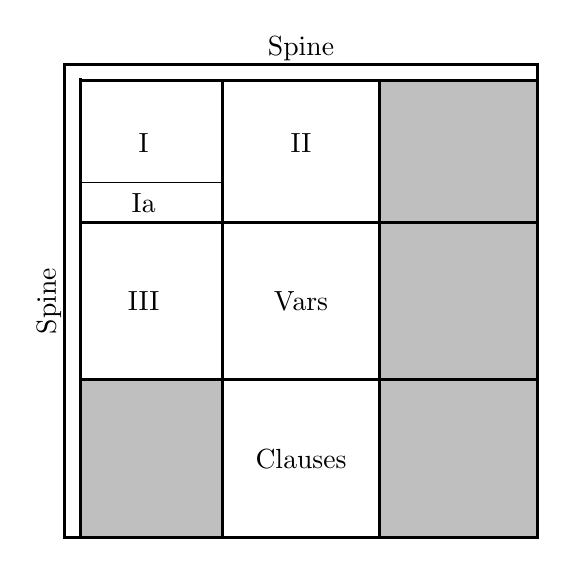
\begin{tikzpicture}
    \colorlet{fill}{gray!50}
    \colorlet{blank}{white}
    \fill[color=fill] (4,0) rectangle (6,-2);
    \fill[color=fill] (4,-2) rectangle (6,-6);
    \fill[color=fill] (0,-4) rectangle (2,-6);
    \draw[very thick, step=2] (0, 0) grid (6, -6);
    \draw (0,-1.5) -- (2,-1.5);
    \fill[color=white] (0,0) rectangle (0.2, -6);
    \fill[color=white] (0, 0) rectangle (6, -0.2);


    \draw[very thick, step=2] (0.2, -0.2) rectangle (0.2, -6);
    \draw[very thick, step=2] (0.2, 0) rectangle (6, -0.2);
    \fill[color=white] (0, 0) rectangle (6, -0.17);

    \draw[very thick, step=2] (0, 0) rectangle (6, -6);


    \node at (1,-1)    {I};
    \node at (1,-1.75) {Ia};
    \node at (1,-3)    {III};
    \node at (3,-1)    {II};
    \node at (3,-3)    {Vars};
    \node at (3,-5)    {Clauses};
    \node[rotate=90] at (-0.2, -3)  {Spine};
    \node at (3, 0.2)  {Spine};
  \end{tikzpicture}
  \caption{Regions of play for a `normal' game.}\label{fig:regions}
\end{figure}
where each `block' is a square $n \times n$ with $n = 2k + 1$.

\begin{theorem}
  In the perfect strategy for Rose, she plays the spine first.
  \begin{proof}
    Consider what happens if she does not. She has two choices for the
    first character. If she chooses a 0, then Colin has a quick kill
    with his bomb regex:
    \begin{figure}[H]
      \centering
      \begin{subfigure}[c]{0.2\textwidth}
        \centering
        \drawgrid{
          {     0, ?, ?, \ldots},
          {     2, , , },
          {     2, , ,},
          {     \vdots, , , },
        }
      \end{subfigure}
      \begin{subfigure}[c]{0.1\textwidth}
        $\xRightarrow[\text{Spine}]{\text{Rose plays}}$
      \end{subfigure}
      \begin{subfigure}[c]{0.2\textwidth}
        \centering
        \drawgrid{
          {     0, ?, ?, \ldots},
          {     2, 1, 0, },
          {     2, , ,},
          {     \vdots, , , },
        }
      \end{subfigure}
      \begin{subfigure}[c]{0.1\textwidth}
        $\xRightarrow[\text{I or II}]{\text{Colin plays}}$
      \end{subfigure}
      \begin{subfigure}[c]{0.2\textwidth}
        \centering
        \drawgrid{
          {     0, ?, ?, \ldots},
          {     2, 1, 0, },
          {     2, 0, ,},
          {     \vdots, \vdots, , },
        }
      \end{subfigure}
      \caption{The board after Rose `cheats' with 0 and Colin plays a bomb.}
    \end{figure}
    A similar result will occur if she cheats with a 1:
    \begin{figure}[H]
      \centering
      \begin{subfigure}[c]{0.2\textwidth}
        \centering
        \drawgrid{
          {     1, ?, ?, \ldots},
          {     0, , , },
          {     0, , ,},
          {     \vdots, , , },
        }
      \end{subfigure}
      \begin{subfigure}[c]{0.15\textwidth}
        $\xRightarrow[\text{plays `}\ldots\text{10'}]{\text{eventually Rose}}$
      \end{subfigure}
      \begin{subfigure}[c]{0.2\textwidth}
        \centering
        \drawgrid{
          {     1, 0, ?, \ldots},
          {     ?,  ,  , },
          {     ?, , ,},
          {     \vdots, , , },
        }
      \end{subfigure}
      \begin{subfigure}[c]{0.1\textwidth}
        $\xRightarrow[\text{bomb}]{\text{Colin plays}}$
      \end{subfigure}
      \begin{subfigure}[c]{0.2\textwidth}
        \centering
        \drawgrid{
          {     1, 0, ?, \ldots},
          {     ?, 2,  , },
          {     ?, 2, ,},
          {     \vdots, \vdots, , },
        }
      \end{subfigure}
      \caption{The board after Rose `cheats' with 0 and Colin plays a bomb.}
    \end{figure}
    In either case, Rose would quickly lose.
  \end{proof}
\end{theorem}
Once the spine has been played, it will determine the rest of play, as
Colin is also forced to play his spine (since it is his only regex
starting with 2). Subsequently, Rose is forced to play the her
``calibration'' regex with $i=0$
\begin{figure}[H]
  \caption{TODO: a picture of the pattern that forces play}
\end{figure}

\begin{theorem}$\TQBF \le_p \RCG$
\begin{proof}
  Assume $\phi$ is a boolean formula in \TQBF.
  \begin{description}
    \item[($\bs{\phi}$ satisfiable)]
      Using the definition of \TQBF, we see that if $\phi$ is
      satisfiable then for any index $i$, we can choose an $x_i$ that
      no matter the choice of $y_i$ sets some clause (say, $c_i$) to
      be true. Recall that $S_{iab}$ is constructed from the value of
      $c_i$ at every possible setting of $x_i$ and $y_i$, so given the
      above we know there is some $S_{iab}$ for every index $i$ that
      sets $c_i$ to be true.

      Since Rose must have a 1 in each row of the clause region, she
      is forced to choose each $x_i$ in the variable region to match a
      corresponding $S_{iab}$ of Colin's that also has a 1 in the clause
      region (no matter Colin's choice of $y_i$). However, given the
      above we know she has such a choice. This means that play will
      continue up until the padding region in the right third of $X$,
      where Colin is now forced to play only $\bs{0}^*$. All of Rose's
      regular expressions allow him to do so until the last column,
      which is now already filled with a string matching
      $\bs{1}\bs{0}^*$. Since this does not match $C$, Colin loses.
    \item[($\bs{\phi}$ unsatisfiable)]
      Since $\phi$ is unsatisfiable, Rose no longer has a choice for
      each $x_i$ that guarantees a 1 in the clause region. Since $R$
      requires that every row in the clause region has a 1, Rose will
      be unable to move and Colin wins.
  \end{description}
  %\begin{align*}
  %  \varphi \text{ is satisfiable} &\iff (\forall i) \; (\exists a) \; (\forall b) \; c_i[x_i \coloneqq a; y_i \coloneqq b] = 1 \\
  %                                 &\iff (\forall i) \; \exists S_{iab} \text{ that sets } c_i = 1 \\
  %                                 &\iff \text{ every row in the clause region contains a } 1 \\
  %                                 &\iff \text{ Rose is the last to move }
  %\end{align*}
\end{proof}
\end{theorem}
\end{document}
